\documentclass[twocolumn,10pt]{jarticle}
\usepackage[dvipdfmx]{graphicx}
\usepackage[top=15truemm,bottom=15truemm,left=13truemm,right=13truemm]{geometry}

\title{\vspace{-1.5cm}\normalsize {\textbf {DAOにおける内部告発の提案}}}
\author{\vspace{-1.1cm} \normalsize	情報・通信工学科 荒木研究室所属 182C1117 津田匠貴}
\date{}
\begin{document}
\vspace{-10pt}
\maketitle

%1-----------------------------------------------------------------------------------------------------------
\vspace{-0.55cm}
\section{\normalsize はじめに}
\vspace{-0.2cm}
DAO(Decentralized Autonomous Organization:自律分散型組織)は共通目的を持った匿名個人らが中央集権的な管理主体を持たず
に経済活動を行う組織であり, 独自トークンの発行や分散台帳としての記録機能をもつブロックチェーン技術の使用を前提に成り立っている.
このような組織が運営する分散的サービスはWeb3.0と呼ばれる.これに対し,特定の企業が中央集権的に運営するTwitterなどの従来のサービスはWeb2.0と呼ばれる.
Web3.0上の組織であるDAOには 検閲耐性があり誰でも匿名で参加できるといったメリットがある一方,自律分散型的に機能するまでは株式会社などの中央集権的組織が主体となって運営しており,彼らによる資金の持ち逃げといった問題が数多く発生している.
このような不正を防止し,コミュニティによる分散的統治を補助するために,本研究ではEthereumブロックチェーンにおいて秘密分散法を用いたメンバーシップの導入と内部告発機能を提案する.
これは不正を行う兆候があるユーザーを検知した場合に内部告発を行い,メンバーの投票による審議を行うことで,不正を防止するスキームを目指している.
%2-----------------------------------------------------------------------------------------------------------
\vspace{-0.55cm}
\section{\normalsize Ethereum}
\vspace{-0.2cm}
Ethereumは暗号資産の移転・管理を誰でもプログラム可能にするスマートコントラクトを実装している.
すでに多くのアプリケーションがこの上に構築されており,これらはいずれも同じプロトコル上で動くため, 相互に連携させることも容易である.
このような汎用性と相互運用性の観点から他のブロックチェーンと比べても巨大なエコシステムを持っている.そのため新しいDAOをEthereum上に組織するプロジェクトが多い.
本研究でも,このような背景からEthereum上のDAOを対象とする.
%3-----------------------------------------------------------------------------------------------------------
\vspace{-0.55cm}
\section{\normalsize 秘密分散法}
\vspace{-0.2cm}
秘密分散法とはある秘密をshareと呼ばれる欠片に分割し複数のメンバーで管理する方式である.本研究では事前に定めた閾値以上のshareが集まった場合にのみ復元できる閾値型秘密分散法を用いたメンバーシップを提案する.
この手法では, ある多項式上の点をshareとし, それを各メンバーに配布するディーラーの存在を仮定している.閾値以上のshareが集まった場合に多項式を復元することができ,秘密を復号することができる.
%4-----------------------------------------------------------------------------------------------------------
\vspace{-0.55cm}
\section{\normalsize DAOにおける内部告発の矛盾点とその解決方法}
\vspace{-0.2cm}
DAOにおいて内部告発を実現する場合, 不正の疑いがあるメンバーを特定する行為は, 匿名環境下での活動と矛盾する.
また,内部告発の対象となる資金の持ち逃げをされた場合, 資金を取り戻すことはほぼ不可能であるため,インシデントが起きる前に不正を防ぐ必要がある.
そのような不正をWeb3.0上の取引から事前に察知するのは困難だが, Web2.0上のチャット内容などから推測できる.そこで本研究では,予めこれらのWeb2.0上のアカウントとWeb3.0上のアカウントを紐付けるメンバーシップを考案した.
これにより,告発によってWeb2.0上のアカウントが公開され, メンバーによる判決結果から有害と認められた場合にのみ, 被告発者のWeb3.0上のアカウントを特定し罰則を与えることができる.
このスキームでは,不正を行おうとすればリスクを負うため,そのような行いを起こそうとするメンバーに対する牽制や,上述の矛盾を緩和することができる.
%5-----------------------------------------------------------------------------------------------------------
\vspace{-0.55cm}
\section{\normalsize 閾値型秘密分散法を用いたメンバーシップ}
\vspace{-0.2cm}
図1は上述のスキームをEthereum上で実現するために考案したアカウント管理モデルである.
\begin{figure}[htbp]
  \begin{center}
    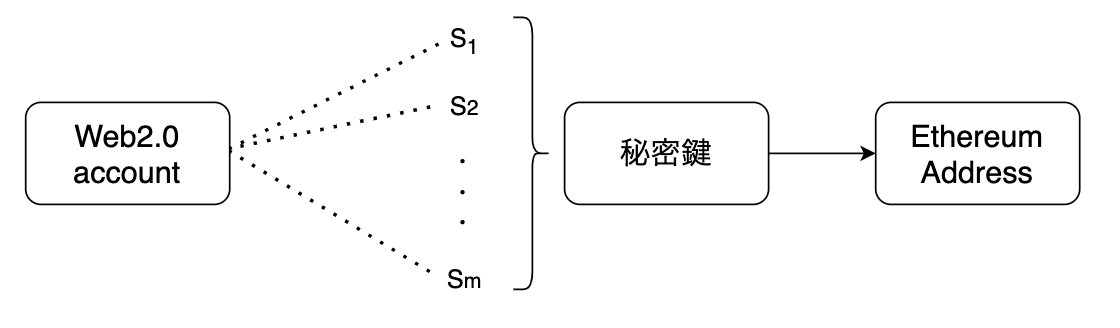
\includegraphics[width=80mm]{share.png}
    \caption{アカウント管理モデル}
  \end{center}
\end{figure}
\vspace{-0.55cm}

全てのメンバーは以下の流れに従いアカウントを登録する.

\begin{enumerate}
  \vspace{-5pt}
  \item アドレスを作成する際に使った秘密鍵を閾値型秘密分散法に基づいて$m$個のshareに分割する\vspace{-5pt}
  \item 1つのWeb2.0 accountにつき, $m$個のshareを紐付けたペアを作る\vspace{-5pt}
  \item それぞれのペアを$m$人のメンバーに配る\vspace{-5pt}
\end{enumerate}

閾値型秘密分散法により$n$個以上のペアが集まれば,被告発者自身の秘密鍵が復元され,アドレス上の資産を失うなどのリスクを負うことになる.
このようなリスクを回避する唯一の方法は,自身が内部告発の対象にならないことでありWeb2.0上で誠実な振る舞いを続け, DAOに危害を与えるような言動を慎むことである.
また,内部告発とメンバーによる審議および制裁のコントロールはスマートコントラクトを用いて行う.
%6-----------------------------------------------------------------------------------------------------------
\vspace{-0.55cm}
\section{\normalsize まとめ・今後の展望}
\vspace{-0.2cm}
本研究では, DAOのコアメンバーによる資金の持ち逃げといった不正を防止する内部告発の準備として閾値型秘密分散法を用いたアカウント管理モデルを提案した.
これにより各メンバーは資産の損失リスクを負った状態で活動するため, 言動に責任を持たせることができる.
しかし, 利用を想定している一般的な閾値型秘密分散法では, ディーラーの存在を仮定しているため, DAOのメリットである自立分散性を損なう形になっている.
そこでまずは, DKGを組み込むことで分散環境に適したスキームを再設計する.
また, ペアの増減や,結託攻撃に対応するために,今後はプロアクティブ秘密分散法や属性ベース暗号による改良も試みる.
\end{document}
